\chapter{Methodology / Research Methodology/ Experimental Methodology / Analytical Methodology/Descriptive Methodology /Case Study Methodology  / Quantitative Research Methodology}


Select any suitable title fro this topic based on your project
	
	\section{Introduction to Methodology}
	\textbf{Purpose:} The objective of the Methodology chapter is to describe the research approach and methods used to address the project objectives.
	
	\textbf{Context:} This section provides a brief overview of the project and explains its significance in the context of the field of study.
	
	\section{Research Design}
	\textbf{Describe Research Design:} The overall research design adopted for the project is \textit{[insert type of research design]} (e.g., experimental, analytical, descriptive, case study).
	
	\textbf{Justification:} This research design was chosen because \textit{[provide reasons why this design aligns with the project goals]}.
	
	\section{Research Approach}
	\textbf{Explain Approach:} The approach used to collect data or information is \textit{[insert type of research approach]} (e.g., quantitative, qualitative, mixed-methods).
	
	\textbf{Rationale:} This approach was selected based on \textit{[explain how it aligns with the research questions and objectives]}.
	
	\section{Sampling Strategy}
	\textbf{Define Sampling:} The sampling technique used is \textit{[describe sampling technique]} (e.g., random sampling, purposive sampling).
	
	\textbf{Sample Size:} The sample size of \textit{[specify sample size]} was chosen to \textit{[justify representativeness or reliability]}.
	
	\section{Data Collection Methods}
	\textbf{Detail Data Collection:} Data was gathered using \textit{[describe data collection methods]} (e.g., surveys, interviews, experiments, observations).
	
	\textbf{Instruments Used:} The tools and instruments utilized include \textit{[mention specific tools or technologies]}.
	
	\section{Data Analysis Techniques}
	\textbf{Outline Analysis Methods:} Collected data will be analyzed using \textit{[explain analysis methods]} (e.g., statistical analysis, thematic analysis, content analysis).
	
	\textbf{Software Tools:} Analysis will be conducted using \textit{[mention software tools or packages]} (e.g., SPSS, MATLAB, NVivo).
	
	\section{Research Ethics}
	\textbf{Ethical Considerations:} Ethical issues related to data collection, participant consent, and confidentiality were addressed by \textit{[explain ethical considerations]}.
	
	\textbf{Compliance:} The research adheres to ethical guidelines and regulations set by \textit{[mention relevant regulatory bodies]}.
	
	\section{Limitations and Assumptions}
	\textbf{Identify Limitations:} Potential limitations in the research approach or methods include \textit{[acknowledge limitations]}.
	
	\textbf{Discuss Assumptions:} Assumptions made during the research process are \textit{[state assumptions]}.
	
	\section{Validation and Reliability}
	\textbf{Ensure Validity:} Steps taken to ensure validity and reliability include \textit{[describe validation methods]} (e.g., triangulation, pilot testing).
	
	\section{Timeline and Schedule}
	\textbf{Project Timeline:} A brief timeline outlining the sequence of research activities and milestones is provided in \textit{[include project timeline]}.
	
	\textbf{Gantt Chart (Optional):} A Gantt chart or schedule diagram can be included to visualize the project timeline.
	
	\section{Writing Tips}
	\begin{itemize}
		\item Use clear and concise language to describe each methodological aspect.
		\item Provide sufficient detail for readers to understand the research process and its rationale.
		\item Include citations to relevant sources to support methodological choices.
		\item Organize the chapter logically, following a structured format from general to specific details.
	\end{itemize}
	





%%%%%%%%%%%%%%%%%%%%%%%%%%%%%%%%%%%%%%%%%%%%%%%%%%%%%%%%
%%%%% for Quick help  folloowng lien are useful
%%%%%%%%%%%%%%%%%%%%%%%%%%%%%%%%%%%%%%

Study the \LaTeX\ code in chapt3.tex.
It will help you for figure insertion, math using \LaTeX\ .\, Table creation,
citations, labels.
\section{Homomorphic filter} 
 %Morphological filters
By performing simultaneous gray level range compression and contrast enhancement on illumination reflection model,one can improve the appearance of an image by designing a frequency domain procedure~\cite{man87}.
An image $f(x,y)$ can be expressed as a product of illumination and reflection components~\cite{sam09}.

 % NOTE2: pl.refer that  $ $ sign for mathamatical term in the text in line.

\begin{equation}
f(x,y)=i(x,y)r(x,y)
\end{equation}

% NOTE3:- \[ f(x,y)=i(x,y)r(x,y) \]
% this has the same effect as above code i.e
%  \begin{equation}
% f(x,y)=i(x,y)r(x,y)
% \end{equation}

here $ i(x,y) $ is  illumination component and  $ r(x,y) $ reflection component.\\

% NOTE 4: Observe the  \\  at the end
% this will help the latex to go to new line.


Fourier transform of the product of two functions is not separable, So we can define shown in as shown in Equation~\ref{fourier}

\begin{equation}
F.T[z(x,y)]=F.T[ln f(x,y)]=F.T[ln i(x,y)]+F.T[ln r(x,y)]
\label{fourier}
\end{equation}

\begin{equation}
Z(u,v)=F_{i}(u,v)+F_{r}(u,v)
\end{equation}


 \begin{equation}
  S(u,v)=H(u,v)Z(u,v)
 \end{equation}

% Note5: Observe the following code ,
% here for the equatins \[                      \] brackets are used
% this will help you if you are not interested in numbering of the equations.
% observe the effect in output pdf file.


 where $S(u,v)$ Fourier Transform of result  and $H(u,v)$ Filter function

      \[S(u,v)=H(u,v)F_{i}(u,v)+H(u,v)F_{r}(u,v)\]

      \[s(x,y)=F^{-1}[S(u,v)]\]

      \[s(x,y)=F^{-1}[H(u,v)F_{i}(u,v)]+F^{-1}[H(u,v)F^{r}(u,v)]\]

      Say
      \[i'(x,y)=F^{-1}[H(u,v)F_{i}(u,v)]\]

       \[r'(x,y)=F^{-1}[H(u,v)F_{r}(u,v)]\]

       Hence,
       \[s(x,y)=i'(x,y)+r'(x,y)\]

       Therefore,
       Let $g(x,y)$ be the inverse exponential operation

       \[g(x,y)=e^{s(x,y)}\]

      \[g(x,y)=e^{i'(x,y)}e^{r'(x,y)}\]

       \[g(x,y)=i_{0}(x,y)+r_{0}(x,y)\]

       where $i_{0}(x,y)=e^{i'(x,y)}$ and $r_{0}(x,y)=e^{r'(x,y)}$


%  Note 6:following five lines are responsible for graphics insertion.

\begin{figure}[h]
	\centering
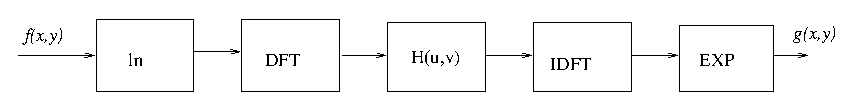
\includegraphics{blockdig.eps}
\caption{Block digram}
	\label{bbb}
\end{figure}

\begin{itemize}
\item This approach is used for homomorphic filtering as shown in figure~\ref{bbb}. The key to the approach is separation of the illumination and reflection components. Between them $i(x,y)$ contributes to the low frequency since illumination is more or less uniform and $r(x,y)$ is high frequency component as it tends to vary abruptly at junctions of dissimilar objects.
\item $H(u,v)$ is the homomorphic filtering function.A typical homomorphic filter $H(u,v)$ is as shown in figure below. Generally, $\gamma_L<1$ and$\gamma_H>1$, $H(u,v)$ tends to decrease the contribution made by low frequencies and amplify the contribution made by high frequency.
\end{itemize}

%NOTE 7: The following five lines are responsible for graphics insertion.
% Also note that in caption q312 is the figure number and after : put name of the figure.

\begin{figure}[htbp]
\centering
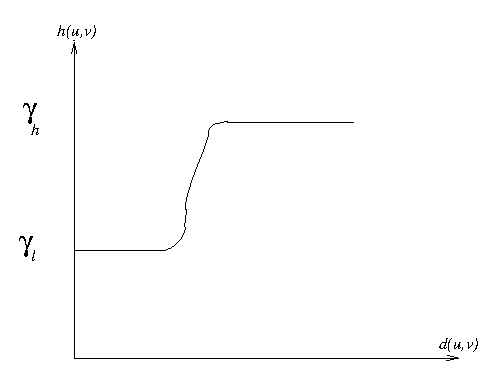
\includegraphics{graph.eps}
\caption{Transfer function}
\label{fig:graph}
\end{figure}

\section{Morphological Filters}

To understand morphological filters we first need to understand the operations dilation, erosion,opening  and  closing.

\subsection{Dilation}
With $A$ and $B$ as sets in $Z^{2}$,the dilation of $A$ and $B$ denoted as $A\oplus B$ is defined as

\[A\oplus B={Z/(\hat{B}_{z}\cap A \neq \phi}\]

Equation obtained by reflection of $B$ about origin and shifting reflection by $ z$ .
$B$  and $A$ should overlap by at least one element.Set $B$ is the structuring element in all morphological operations.\\
 \textbf{Erosion} For sets $A$ and $B$ in $Z^{2}$,the erosion of $A$ by $B$ denoted as $A\ominus B$ is defined as

\[ A\ominus B={Z/(B_{z}\subseteq A )} \]
This equation indicates that the erosion of $A$ by $B$ is the set of all points $z$ such that $B$,translated by $z$ is contained in $A$ Erosion shrinks an image.

\subsection{Opening and closing}

Opening smooths the contour of an object.
 Closing also tends to smooth sections of contours but it generally fuses narrow breaks and long thin gulfs,eliminates small holes and fills gaps in contour.
Opening is denoted by $A\circ B$

\[A\circ B=(A\ominus B)\oplus B\]

  i.e. Erosion followed by dilation
 Closing is denoted by $A\bullet B$

 \[A\bullet B=(A\oplus B)\ominus B\]

 i.e Dilation followed by erosion.
 Morphological operations can be used to construct filters.

\begin{enumerate}
	\item Suppose we have a binary image which is corrupted by noise.The noise manifests itself as light elements on a dark background and dark elements on  light components of image .
	\item A morphological filter consisting of opening followed by closing operation eliminates the noise and its effect on the image while distorting it as little as possible.
	\item The steps are as follows

\begin{itemize}
	\item We have a structuring element
	\item We erode A with the structuring element.The background noise gets eliminated in the erosion stage of opening because in this case all noise components are physically smaller then the structuring element.
For e.g. in some images the size of the noise elements actually increases.This is because these elements are inner boundaries that should increase in size as object is eroded.
\item This enlargement is countered by performing dilation.The noise components in the image are reduced in size or deleted completely.
The two operations constitute ~``opening'' A by B.
\item Net effect of opening is to eliminate all noise components in both the background and image itself.However,new gaps may be formed.
\item To counter this effect we perform dilation on the opening.Sometimes most breaks are restored but ridges are thickened.
This thickening is countered by erosion.
\item The above two steps are the closing operation.
\end{itemize}

\end{enumerate}
Hence the final result is remarkably clean of noise specs.
 Disadvantage of this filter is that some of the point ridges might not be fully repaired and can contain breaks. \\

%Note 8: If u want to insert a table your editor will help u to create %a required code for that
% for example refer the following
% go to the wizard menu and use Quick Tabular

The Table~\ref{tab:listOfStudents} is used to explain how table can be created in Latex and also observe how table in the document can be referred  in text.


\begin{table}[htbp]
	\centering
		\begin{tabular}{|c|c|c|}
			\hline Roll No & Name of the student & marks \\
			\hline 1 & Sonal & 95 \\
			\hline 2 & Komal & 97 \\
			\hline
\end{tabular}
\caption{list of students}
\label{tab:listOfStudents}
\end{table}




%Note9 With a little pactice of this code you will get the idea about how to 
% use $ $, \[  \],  \\ ,
% how to insert graphics and  create Tables.
%Note10: If u are creating table of contents, List of Figures,cross reference, Citation, ...,
%then run the same code for two times.